\documentclass[compress]{beamer}
\usepackage[utf8]{inputenc}
\usepackage[T1]{fontenc}

\usepackage{amsfonts}
\usepackage{amsmath}
\usepackage{amssymb}

\title{Symplectic Classification of Simplices}
\date[9. 9. 2019]{bachelor colloquium}
\author[Konstantin Fickel]{Konstantin Fickel \texttt{konstantin.fickel@student.uni-augsburg.de}}
\usetheme{focus}

\begin{document} 

\section{Introduction}

\blankframe{}

\begin{frame} 
  \begin{center}
    \begin{overprint}
      \onslide<1>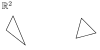
\includegraphics[scale=1.0]{../img/introduction/01.pdf}
      \onslide<2>\includegraphics[scale=1.0]{../img/introduction/02.pdf}
      \onslide<3>\includegraphics[scale=1.0]{../img/introduction/03.pdf}
      \onslide<4>\includegraphics[scale=1.0]{../img/introduction/04.pdf}
      \onslide<5>\includegraphics[scale=1.0]{../img/introduction/05.pdf}
      \onslide<6>\includegraphics[scale=1.0]{../img/introduction/06.pdf}
      \onslide<7>\includegraphics[scale=1.0]{../img/introduction/07.pdf}
      \onslide<8>\includegraphics[scale=1.0]{../img/introduction/08.pdf}
      \onslide<9>\includegraphics[scale=1.0]{../img/introduction/09.pdf}
      \onslide<10>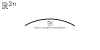
\includegraphics[scale=1.0]{../img/introduction/10.pdf}
      \onslide<11>\includegraphics[scale=1.0]{../img/introduction/11.pdf}
      \onslide<12>\includegraphics[scale=1.0]{../img/introduction/12.pdf}
    \end{overprint}
  \end{center}
\end{frame}

\blankframe{}

\section{Theorem}

\begin{frame}
  \begin{center}
    \begin{overprint}
      \onslide<1>\includegraphics[scale=1.0]{../img/conditions/01.pdf}
      \onslide<2>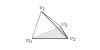
\includegraphics[scale=1.0]{../img/conditions/02.pdf}
      \onslide<3>\includegraphics[scale=1.0]{../img/conditions/03.pdf}
      \onslide<4>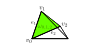
\includegraphics[scale=1.0]{../img/conditions/04.pdf}
      \onslide<5>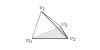
\includegraphics[scale=1.0]{../img/conditions/02.pdf}
      \onslide<6>\includegraphics[scale=1.0]{../img/conditions/05.pdf}
      \onslide<7>\includegraphics[scale=1.0]{../img/conditions/06.pdf}
      \onslide<8>\includegraphics[scale=1.0]{../img/conditions/07.pdf}
      \onslide<9>\includegraphics[scale=1.0]{../img/conditions/08.pdf}
    \end{overprint}
  \end{center}
\end{frame}
\begin{frame}{(3) Border of 3-simplices}
  \begin{center}
    \begin{overprint}
      \onslide<1>\includegraphics[scale=1.0]{../img/conditions/09.pdf}
    \end{overprint}
  \end{center}
\end{frame}
\begin{frame}
  \begin{center}
    \begin{overprint}
      \onslide<1>\includegraphics[scale=1.0]{../img/conditions/10.pdf}
      \onslide<2>\includegraphics[scale=1.0]{../img/conditions/11.pdf}
      \onslide<3>\includegraphics[scale=1.0]{../img/conditions/12.pdf}
    \end{overprint}
  \end{center}
\end{frame}

\bgroup
\setbeamercovered{invisible}
\setbeamercovered{%
again covered={\opaqueness<1->{50}}}
\begin{frame}{(4) Nondegeneracy}
  \begin{align*}
    0 \neq \nu_{1, \dots, 2n} & \onslide<2-3>{= \frac{1}{n!} \cdot \omega^{n} \left( e_1, \dots, e_{2n} \right)} \\ & \onslide<3-4>{= \frac{1}{n!\cdot2^n} \sum\limits_{\pi \in S_n} \left( \prod\limits_{k=1}^{n} \omega \left( e_{\pi \left(2k-1\right)}, e_{\pi \left(2k\right)} \right) \right)} \\
                              & \onslide<4-5>{= \frac{1}{n!\cdot2^n} \sum\limits_{\pi \in S_n} \left( \prod\limits_{k=1}^{n} \nu_{\pi \left(2k-1\right), \pi \left(2k\right)} \right)}
  \end{align*}
\end{frame}
\egroup

\blankframe{}

\section{Recursion Formula}

\begin{frame}
  \begin{center}
    \begin{overprint}
      \onslide<1>\includegraphics[scale=1.0]{../img/recursionformula/01.pdf}
      \onslide<2>\includegraphics[scale=1.0]{../img/recursionformula/02.pdf}
      \onslide<3>\includegraphics[scale=1.0]{../img/recursionformula/03.pdf}
      \onslide<4>\includegraphics[scale=1.0]{../img/recursionformula/04.pdf}
      \onslide<5>\includegraphics[scale=1.0]{../img/recursionformula/05.pdf}
      \onslide<6>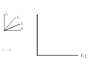
\includegraphics[scale=1.0]{../img/recursionformula/06.pdf}
      \onslide<7>\includegraphics[scale=1.0]{../img/recursionformula/07.pdf}
      \onslide<8>\includegraphics[scale=1.0]{../img/recursionformula/08.pdf}
      \onslide<9>\includegraphics[scale=1.0]{../img/recursionformula/09.pdf}
      \onslide<10>\includegraphics[scale=1.0]{../img/recursionformula/10.pdf}
      \onslide<11>\includegraphics[scale=1.0]{../img/recursionformula/11.pdf}
      \onslide<12>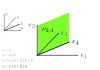
\includegraphics[scale=1.0]{../img/recursionformula/12.pdf}
      \onslide<13>\includegraphics[scale=1.0]{../img/recursionformula/13.pdf}
      \onslide<14>\includegraphics[scale=1.0]{../img/recursionformula/14.pdf}
    \end{overprint}
  \end{center}
\end{frame}

\blankframe{}

\begin{frame}
\begin{overprint}
\onslide<1>
\begin{equation*}
  \tiny
  \rho_{j,i} = \left\lbrace
\begin{array}{llr}
  1 & \textnormal{ for } 2 \nmid j \textnormal{ and } i = j + 1  \textnormal{ and } j \in \left\lbrace 1, \dots, 2n \right\rbrace \\
  \frac{\left( -1 \right) ^ i}{\rho_{i, \sigma\left( i \right)}} \left( \nu_{i,j} + \sum \limits _{m=1} ^{2k-2} \left( -1 \right) ^m \rho_{i, m} \cdot \rho_{j, \sigma \left( m \right)} \right) &\textnormal{ for } 1 \leq i < j \leq 2n \textnormal { with } i = 2k \lor i=2k-1 \\
  0 & \textnormal{otherwise}
\end{array}
\right.
\end{equation*}
\onslide<2>
\begin{equation*}
  \tiny
  \rho_{j,i} = \left\lbrace
\begin{array}{llr}
  1 & \textnormal{ for } 2 \nmid j \textnormal{ and } i = j + 1  \textnormal{ and } j \in \left\lbrace 1, \dots, 2n \right\rbrace \\
  \frac{\left( -1 \right) ^ i}{{\color{red} \rho_{i, \sigma\left( i \right)}}} \left( \nu_{i,j} + \sum \limits _{m=1} ^{2k-2} \left( -1 \right) ^m \rho_{i, m} \cdot \rho_{j, \sigma \left( m \right)} \right) &\textnormal{ for } 1 \leq i < j \leq 2n \textnormal { with } i = 2k \lor i=2k-1 \\
  0 & \textnormal{otherwise}
\end{array}
\right.
\end{equation*}
\end{overprint}
\end{frame}

\blankframe{}

\begin{frame}
  \begin{equation*}
    \rho_{j,i} = \left\lbrace
  \begin{array}{lr}
    0 & \textnormal{ for } i \geq j \lor i \leq 0 \\
    -\frac{\nu_{1,\dots,2k-2,2k-1,j}}{\nu_{1,\dots,2k-2}} & \textnormal{ for } 0 < i < j \leq 2n \land i = 2k - 1 \textnormal{ with } k \in \mathbb{N} \\
    -\frac{\nu_{1,\dots,2k-2,2k,j}}{\nu_{1,\dots,2k}} & \textnormal{ for } 0 < i < j \leq 2n \land i = 2k \textnormal{ with } k \in \mathbb{N}
  \end{array} \right.
  \end{equation*}
\end{frame}

\begin{frame}
\begin{equation*}
\rho_{i, \sigma \left( i \right)} =
\left\lbrace
\begin{array}{lr}
  \frac{\nu_{1,\dots,i}}{\nu_{1,\dots,i-2}} & 2 \mid i\\
  1 & 2 \nmid i
\end{array}
\right.
\end{equation*}
\end{frame}

\section{Reordering Lemma}

\bgroup
\setbeamercovered{invisible}
\setbeamercovered{%
again covered={\opaqueness<1->{50}}}
\begin{frame}
  \begin{align*}
    \onslide<1-11>{\nu_{1,2} & \neq 0} \\
    \onslide<2-10>{\nu_{1,2,3,4} & \neq 0} \\
    \onslide<2-10>{ & \vdots} \\
    \onslide<2-9>{\nu_{1,2, \dots, 2n-4} & \neq 0} \\
    \onslide<2-8>{\nu_{1,2, \dots, 2n-2} & \neq 0} \\
    \onslide<2-12>{\nu_{1,2, \dots, 2n} & \neq 0}
  \end{align*}
  \vfill
  {
    \small
    \begin{align*}
      \onslide<3->{0 & \neq} \onslide<3-4>{\omega^{k} \left( e_1, \dots, e_{2k} \right)} \onslide<4-5>{= \omega^{k-1} \wedge \omega \left( e_1, \dots, e_{2k} \right)} \\
                     & \onslide<5-6>{= \frac{1}{\left(2k - 2\right)! \cdot 2!} \cdot \sum \limits_{\tau \in S_{2k}} \textnormal{sgn} \left( \tau \right)} \onslide<5->{\omega^{k-1} \left( e_{\tau \left( 1 \right)}, \dots, e_{\tau \left( 2k - 2 \right)} \right)} \onslide<5-6>{\cdot \omega \left( e_{\tau \left( 2k-1 \right)}, e_{\tau \left( 2k \right)} \right)}
    \end{align*}
  }
\end{frame}
\egroup

\blankframe{}
\end{document}

